\documentclass{standalone}
\usepackage{tikz}
\usetikzlibrary{patterns, positioning}

\begin{document}
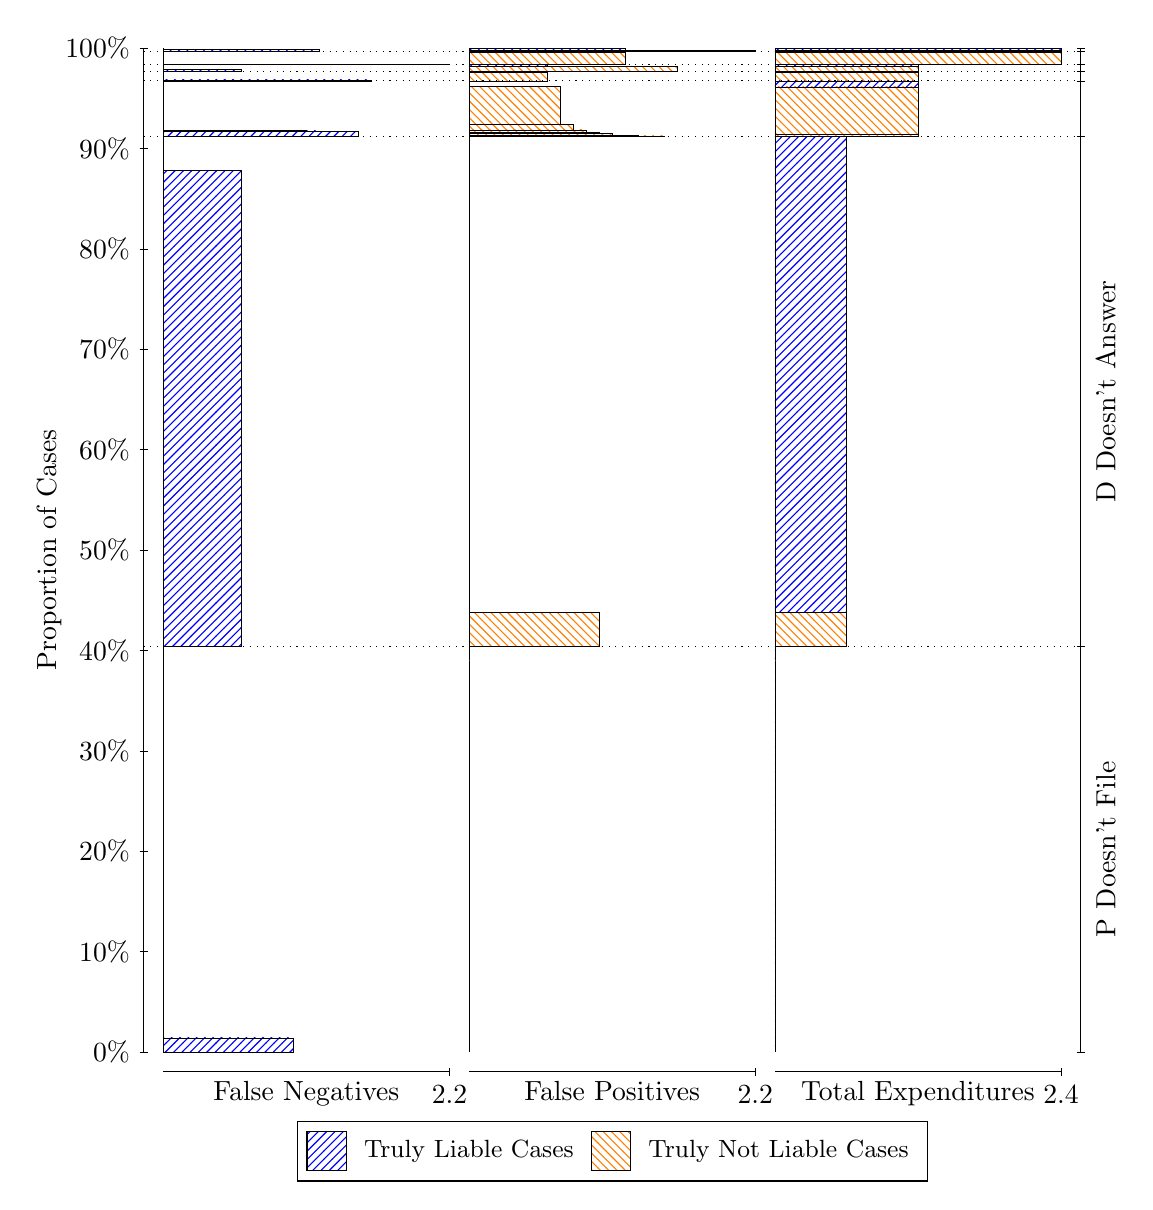
\begin{tikzpicture}
\draw[black, very thin] (1.5,1.75) -- (1.5,14.5);
\node[rotate=90, anchor=center] at (0.3, 8.125) {Proportion of Cases};
\draw[black, very thin] (1.45,1.75) -- (1.55,1.75);
\node[anchor=east] at (1.45, 1.75) {0\%};
\draw[black, very thin] (1.45,3.025) -- (1.55,3.025);
\node[anchor=east] at (1.45, 3.025) {10\%};
\draw[black, very thin] (1.45,4.3) -- (1.55,4.3);
\node[anchor=east] at (1.45, 4.3) {20\%};
\draw[black, very thin] (1.45,5.575) -- (1.55,5.575);
\node[anchor=east] at (1.45, 5.575) {30\%};
\draw[black, very thin] (1.45,6.85) -- (1.55,6.85);
\node[anchor=east] at (1.45, 6.85) {40\%};
\draw[black, very thin] (1.45,8.125) -- (1.55,8.125);
\node[anchor=east] at (1.45, 8.125) {50\%};
\draw[black, very thin] (1.45,9.4) -- (1.55,9.4);
\node[anchor=east] at (1.45, 9.4) {60\%};
\draw[black, very thin] (1.45,10.675) -- (1.55,10.675);
\node[anchor=east] at (1.45, 10.675) {70\%};
\draw[black, very thin] (1.45,11.95) -- (1.55,11.95);
\node[anchor=east] at (1.45, 11.95) {80\%};
\draw[black, very thin] (1.45,13.225) -- (1.55,13.225);
\node[anchor=east] at (1.45, 13.225) {90\%};
\draw[black, very thin] (1.45,14.5) -- (1.55,14.5);
\node[anchor=east] at (1.45, 14.5) {100\%};

\draw[black, very thin] (13.4,1.75) -- (13.4,14.5);
\draw[black, very thin] (13.35,1.75) -- (13.45,1.75);
\node[anchor=west] at (13.35, 1.75) {};
\draw[black, very thin] (13.35,6.8993) -- (13.45,6.8993);
\node[anchor=west] at (13.35, 6.8993) {};
\draw[black, very thin] (13.35,13.381) -- (13.45,13.381);
\node[anchor=west] at (13.35, 13.381) {};
\draw[black, very thin] (13.35,14.083) -- (13.45,14.083);
\node[anchor=west] at (13.35, 14.083) {};
\draw[black, very thin] (13.35,14.207) -- (13.45,14.207);
\node[anchor=west] at (13.35, 14.207) {};
\draw[black, very thin] (13.35,14.288) -- (13.45,14.288);
\node[anchor=west] at (13.35, 14.288) {};
\draw[black, very thin] (13.35,14.455) -- (13.45,14.455);
\node[anchor=west] at (13.35, 14.455) {};
\draw[black, very thin] (13.35,14.5) -- (13.45,14.5);
\node[anchor=west] at (13.35, 14.5) {};

\draw[black, very thin, pattern color=blue, pattern=north east lines] (1.75,1.75) rectangle (3.4015,1.9296);
\draw[black, very thin, pattern color=orange, pattern=north west lines] (1.75,1.9296) rectangle (1.75,6.8993);
\draw[black, very thin, pattern color=blue, pattern=north east lines] (1.75,6.8993) rectangle (2.7409,12.946);
\draw[black, very thin, pattern color=orange, pattern=north west lines] (1.75,12.946) rectangle (1.75,13.381);
\draw[black, very thin, pattern color=blue, pattern=north east lines] (1.75,13.381) rectangle (4.2273,13.437);
\draw[black, very thin, pattern color=blue, pattern=north east lines] (1.75,13.437) rectangle (4.0621,13.443);
\draw[black, very thin, pattern color=blue, pattern=north east lines] (1.75,13.443) rectangle (3.897,13.446);
\draw[black, very thin, pattern color=blue, pattern=north east lines] (1.75,13.446) rectangle (3.7318,13.449);
\draw[black, very thin, pattern color=blue, pattern=north east lines] (1.75,13.449) rectangle (3.5667,13.451);
\draw[black, very thin, pattern color=blue, pattern=north east lines] (1.75,13.451) rectangle (3.4015,13.452);
\draw[black, very thin, pattern color=blue, pattern=north east lines] (1.75,13.452) rectangle (3.2364,13.453);
\draw[black, very thin, pattern color=blue, pattern=north east lines] (1.75,13.453) rectangle (3.0712,13.454);
\draw[black, very thin, pattern color=blue, pattern=north east lines] (1.75,13.454) rectangle (2.9061,13.455);
\draw[black, very thin, pattern color=orange, pattern=north west lines] (1.75,13.455) rectangle (1.75,14.083);
\draw[black, very thin, pattern color=blue, pattern=north east lines] (1.75,14.083) rectangle (4.3924,14.096);
\draw[black, very thin, pattern color=orange, pattern=north west lines] (1.75,14.096) rectangle (1.75,14.207);
\draw[black, very thin, pattern color=blue, pattern=north east lines] (1.75,14.207) rectangle (2.7409,14.233);
\draw[black, very thin, pattern color=orange, pattern=north west lines] (1.75,14.233) rectangle (1.75,14.288);
\draw[black, very thin, pattern color=blue, pattern=north east lines] (1.75,14.288) rectangle (5.3833,14.293);
\draw[black, very thin, pattern color=orange, pattern=north west lines] (1.75,14.293) rectangle (1.75,14.455);
\draw[black, very thin, pattern color=blue, pattern=north east lines] (1.75,14.455) rectangle (3.7318,14.486);
\draw[black, very thin, pattern color=orange, pattern=north west lines] (1.75,14.486) rectangle (1.75,14.5);
\draw[black, very thin, pattern color=orange, pattern=north west lines] (5.6333,1.75) rectangle (5.6333,6.7197);
\draw[black, very thin, pattern color=blue, pattern=north east lines] (5.6333,6.7197) rectangle (5.6333,6.8993);
\draw[black, very thin, pattern color=orange, pattern=north west lines] (5.6333,6.8993) rectangle (7.2848,7.3349);
\draw[black, very thin, pattern color=blue, pattern=north east lines] (5.6333,7.3349) rectangle (5.6333,13.381);
\draw[black, very thin, pattern color=orange, pattern=north west lines] (5.6333,13.381) rectangle (8.1106,13.383);
\draw[black, very thin, pattern color=orange, pattern=north west lines] (5.6333,13.383) rectangle (7.9455,13.385);
\draw[black, very thin, pattern color=orange, pattern=north west lines] (5.6333,13.385) rectangle (7.7803,13.389);
\draw[black, very thin, pattern color=orange, pattern=north west lines] (5.6333,13.389) rectangle (7.6152,13.394);
\draw[black, very thin, pattern color=orange, pattern=north west lines] (5.6333,13.394) rectangle (7.45,13.412);
\draw[black, very thin, pattern color=orange, pattern=north west lines] (5.6333,13.412) rectangle (7.2848,13.43);
\draw[black, very thin, pattern color=orange, pattern=north west lines] (5.6333,13.43) rectangle (7.1197,13.461);
\draw[black, very thin, pattern color=orange, pattern=north west lines] (5.6333,13.461) rectangle (6.9545,13.532);
\draw[black, very thin, pattern color=orange, pattern=north west lines] (5.6333,13.532) rectangle (6.7894,14.009);
\draw[black, very thin, pattern color=blue, pattern=north east lines] (5.6333,14.009) rectangle (6.4591,14.01);
\draw[black, very thin, pattern color=blue, pattern=north east lines] (5.6333,14.01) rectangle (6.2939,14.011);
\draw[black, very thin, pattern color=blue, pattern=north east lines] (5.6333,14.011) rectangle (6.1288,14.012);
\draw[black, very thin, pattern color=blue, pattern=north east lines] (5.6333,14.012) rectangle (5.9636,14.013);
\draw[black, very thin, pattern color=blue, pattern=north east lines] (5.6333,14.013) rectangle (5.7985,14.015);
\draw[black, very thin, pattern color=blue, pattern=north east lines] (5.6333,14.015) rectangle (5.6333,14.083);
\draw[black, very thin, pattern color=orange, pattern=north west lines] (5.6333,14.083) rectangle (6.6242,14.193);
\draw[black, very thin, pattern color=blue, pattern=north east lines] (5.6333,14.193) rectangle (5.6333,14.207);
\draw[black, very thin, pattern color=orange, pattern=north west lines] (5.6333,14.207) rectangle (8.2758,14.262);
\draw[black, very thin, pattern color=blue, pattern=north east lines] (5.6333,14.262) rectangle (6.6242,14.288);
\draw[black, very thin, pattern color=orange, pattern=north west lines] (5.6333,14.288) rectangle (7.6152,14.45);
\draw[black, very thin, pattern color=blue, pattern=north east lines] (5.6333,14.45) rectangle (5.9636,14.455);
\draw[black, very thin, pattern color=orange, pattern=north west lines] (5.6333,14.455) rectangle (9.2667,14.47);
\draw[black, very thin, pattern color=blue, pattern=north east lines] (5.6333,14.47) rectangle (7.6152,14.5);
\draw[black, very thin, pattern color=orange, pattern=north west lines] (9.5167,1.75) rectangle (9.5167,6.7197);
\draw[black, very thin, pattern color=blue, pattern=north east lines] (9.5167,6.7197) rectangle (9.5167,6.8993);
\draw[black, very thin, pattern color=orange, pattern=north west lines] (9.5167,6.8993) rectangle (10.425,7.3349);
\draw[black, very thin, pattern color=blue, pattern=north east lines] (9.5167,7.3349) rectangle (10.425,13.381);
\draw[black, very thin, pattern color=orange, pattern=north west lines] (9.5167,13.381) rectangle (11.333,13.4);
\draw[black, very thin, pattern color=blue, pattern=north east lines] (9.5167,13.4) rectangle (11.333,13.403);
\draw[black, very thin, pattern color=orange, pattern=north west lines] (9.5167,13.403) rectangle (11.333,14.006);
\draw[black, very thin, pattern color=blue, pattern=north east lines] (9.5167,14.006) rectangle (11.333,14.075);
\draw[black, very thin, pattern color=orange, pattern=north west lines] (9.5167,14.075) rectangle (11.333,14.081);
\draw[black, very thin, pattern color=blue, pattern=north east lines] (9.5167,14.081) rectangle (11.333,14.083);
\draw[black, very thin, pattern color=orange, pattern=north west lines] (9.5167,14.083) rectangle (11.333,14.193);
\draw[black, very thin, pattern color=blue, pattern=north east lines] (9.5167,14.193) rectangle (11.333,14.207);
\draw[black, very thin, pattern color=orange, pattern=north west lines] (9.5167,14.207) rectangle (11.333,14.262);
\draw[black, very thin, pattern color=blue, pattern=north east lines] (9.5167,14.262) rectangle (11.333,14.288);
\draw[black, very thin, pattern color=orange, pattern=north west lines] (9.5167,14.288) rectangle (13.15,14.45);
\draw[black, very thin, pattern color=blue, pattern=north east lines] (9.5167,14.45) rectangle (13.15,14.455);
\draw[black, very thin, pattern color=orange, pattern=north west lines] (9.5167,14.455) rectangle (13.15,14.47);
\draw[black, very thin, pattern color=blue, pattern=north east lines] (9.5167,14.47) rectangle (13.15,14.5);
\draw[black, dotted] (1.5,6.8993) -- (13.4,6.8993);
\draw[black, dotted] (1.5,13.381) -- (13.4,13.381);
\draw[black, dotted] (1.5,14.083) -- (13.4,14.083);
\draw[black, dotted] (1.5,14.207) -- (13.4,14.207);
\draw[black, dotted] (1.5,14.288) -- (13.4,14.288);
\draw[black, dotted] (1.5,14.455) -- (13.4,14.455);
\draw[black, very thin] (1.75,1.5) -- (5.3833,1.5);
\node[anchor=north] at (3.5667, 1.5) {False Negatives};
\draw[black, very thin] (5.3833,1.45) -- (5.3833,1.55);
\node[anchor=north] at (5.3833, 1.45) {2.2};

\draw[black, very thin] (5.6333,1.5) -- (9.2667,1.5);
\node[anchor=north] at (7.45, 1.5) {False Positives};
\draw[black, very thin] (9.2667,1.45) -- (9.2667,1.55);
\node[anchor=north] at (9.2667, 1.45) {2.2};

\draw[black, very thin] (9.5167,1.5) -- (13.15,1.5);
\node[anchor=north] at (11.333, 1.5) {Total Expenditures};
\draw[black, very thin] (13.15,1.45) -- (13.15,1.55);
\node[anchor=north] at (13.15, 1.45) {2.4};

\node[black, centered, rotate=90] at (13.72, 4.3247) {P Doesn't File};
\node[black, centered, rotate=90] at (13.72, 10.14) {D Doesn't Answer};






\draw (7.449999999999999,1.5) node[draw=none] (baseCoordinate) {};
\begin{scope}[align=center]
        \matrix[scale=0.5, draw=black, below=0.5cm of baseCoordinate, nodes={draw}, column sep=0.1cm]{
            \node[rectangle, draw, minimum width=0.5cm, minimum height=0.5cm, pattern=north east lines, pattern color=blue] {}; &
            \node[draw=none, font=\small] (B) {Truly Liable Cases}; &
            \node[rectangle, draw, minimum width=0.5cm, minimum height=0.5cm, pattern=north west lines, pattern color=orange] {}; &
            \node[draw=none, font=\small] (B) {Truly Not Liable Cases}; \\
            };
\end{scope}

\end{tikzpicture}
\end{document}